\documentclass{homework}
\usepackage{lipsum}
\usepackage{alltt}
\usepackage{cancel}
\usepackage{amsthm}
\usepackage{cleveref}
\usepackage{upgreek}
\usepackage{mathrsfs}
\usepackage{tikz}
\usepackage{units}
\usepackage{slashbox}
\newtheorem{lemma}{Lemma}

\DeclareMathOperator{\cov}{cov}

\title{Kevin Joyce}
\course{Stat 542 - Sampling - Homework 1}
\author{Kevin Joyce}
\docdate{\today}
\begin{document} 
\newcommand{\figref}[1]{\figurename~\ref{#1}}
\renewcommand{\bar}{\overline}
\renewcommand{\hat}{\widehat}
\renewcommand{\SS}{\mathcal S}
\newcommand{\HH}{\mathscr H}
\newcommand{\mom}{\widetilde}
\newcommand{\mle}{\widehat \Uptheta}
\newcommand{\eps}{\varepsilon}
\newcommand{\todist}{\stackrel{D}\longrightarrow}
\newcommand{\toprob}{\stackrel{p}\longrightarrow}
\newcommand{\TTheta}{\overline{\underline \Theta} }
\newcommand{\del}{\partial}
\newcommand{\approxsim}{\overset{\cdotp}{\underset{\cdotp}{\sim}}}
\newcommand{\RSS}{\ensuremath{\mathrm{RSS}}}
\newcommand{\MSE}{\ensuremath{\mathrm{MSE}}}
\newcommand{\SE}{\ensuremath{\mathrm{SE}}}
\newcommand{\TSS}{\ensuremath{\mathrm{TSS}}}
\newcommand{\Var}{\ensuremath{\mathrm{Var}}}
\newcommand{\SSReg}{\ensuremath{\mathrm{SSReg}}}
\renewcommand{\a}[1]{{\color{red} \it #1}}

\problem{From the ``Sampling Problems'' on pp. 6-7 of the notes, give the sampling unit, population, sampling plan for each stage of sampling for problem 1, all parts.  Be specific in your answers.}

%\begin{enumerate}
%  \item 
  A researcher has a list of all 4-year colleges and universities in the United States.  
  \begin{enumerate}[(a)]
    \item The parameter of interest is the proportion of 4-year schools which offer a degree in education.  The names of 50 schools are drawn at random from the list and the proportion of these 50 offering such a degree is computed.
    \begin{solution}
      The sampling unit is a school (4-year college or university) with the population being all such schools in the United States.  This is a one-stage simple random sample (SRS).
    \end{solution}
    \item As in $(a)$, but the list is divided into three groups according to enrollment: less than 2000 students, 2000 to 10000 students, greater than 10000 students.  Twenty schools are drawn at random from each group.
    \begin{solution} 
    This is a stratified two-stage sampling plan.  At the first stage, the sampling unit is school-size-group with the population being each of the three groups and the plan is a census.  At the second stage, the sampling unit is a school with the population being schools in a given size-group and the plan is a SRS.
    \end{solution}
    \item The groups in (b) are each subdivided into two groups: those which offer graduate degrees (in any field) and those which do not.  Ten schools are drawn at random from each of these subgroups.
    \begin{solution}
    This adds an intermediate stage to the two in (b).  The first stage is the same, the second stage has binary sampling unit of graduate-degree-granting-status given a school-size group and the plan is again a census.  In the third stage, the sampling unit is a school, and the population is the collection of schools with a given school-size group and a graduate-degree-granting status. The third stage plan is again a SRS.
    \end{solution}
    \item The parameter of interest is the average age of full-time students in all the schools.  Fifty schools are drawn at random and the average age of all students at these 50 schools is computed.
    \begin{solution}
    This is a two-stage cluster sample.  At the first stage, the sampling unit is a school being drawn from the population of all schools in the US, and the plan is a SRS.  At the second stage, the sampling unit is a student from the sampling population of all students at a given school, and it is a census.
    \end{solution}
    \item As in (d), except that 100 students are chosen at random from each of the 50 schools and the average age of these students computed.
    \begin{solution}
      This is a two-stage plan. The first stage is as before and the sampling unit and sampling population are the same as before, but the second stage plan is a SRS.
    \end{solution}
  \end{enumerate}
%  \item A researcher wishes to estimate the proportion of bare ground on a 40-acre parcel of land.
%  \begin{enumerate}
%    \item She stands in the ``middle'' of the parcel and randomly chooses five numbers from 1 to 360.  These represent the directions, in degrees from North, of five transects through the middle point which extend to the edges of the parcel.  On each transect, she uses a measuring wheel to determine how much of that transect lies in bare ground.
%    \begin{solution}
%      This is a single stage plane. Integer degree transects (the sampling unit) are selected from $\{1^\circ,2^\circ,\dots,360^\circ\}$ (the sampling population) by a SRS.
%    \end{solution}
%    \item As in (a), except that for each transect she chooses a random distance from $0$ to $5$ meters from the center.  At five-meter intervals along the transect starting at this point, she centers a circle with radius $0.5$ meters.  She does this for all the transects.  She then determines the proportion of bare ground in all the 0.5-meter circles.
%    \begin{solution}
%    This is a two-stage cluster sample.  Each integer degree transect is selected from $\{1^\circ,2^\circ,\dots,360^\circ\}$ is selected by census in the first stage.  In the second stage, 0.5-meter radius circles centered at increments of 0.5-meters are chosen among all such circles of along a given transect are chosen in a systematic random sample.
%    \end{solution}
%    \item Repeat (a),(b), and (c), except that the transects are five parallel North-South lines evenly-spaced across the parcel.
%    \begin{solution}
%    \end{solution}
%  \end{enumerate}
%  \item A researcher is interested in black bears in a certain geographic region, particularly the size of the bears and the amount of time they spend in various habitats during the summer.
%  \begin{enumerate}
%    \item He sets up traps at five locations scattered throughout the region.  He continues trapping until ten bears have been caught.  He estimates average size characteristics from these ten bears.
%    \begin{solution}
%    This is a one stage opportunistic sample where the sampling units are bears and the population is all bears in the region.
%    \end{solution}
%    \item As in (a), but he radio collars the bears.  Each bear is located once each week during the summer at the same time on the same day of the week.  These observations are used to estimate the proportion of time bears spend in various habitats during the summer.
%    \begin{solution}
%    This is a two stage sample.  In the first stage, the sampling units, population and plan are the same as in part (a).  At the second stage, a census is taken of each date-time from the collection of all date times with a given daily time and day of the week in the summer of interest.
%    \end{solution}
%    \item As in (b), but each bear is located at a randomly chosen time on a randomly chosen day during each week.
%    \begin{solution}
%    This is a two stage sample. The first stage is as in (a) and (b).  At the second stage, a SRS of size one is chosen from the sampling population given in (b).
%    \end{solution}
%    \item As in (a), but he radio collars the first five females and the first five males he traps.
%    \begin{solution}
%    This is also opportunistic, but could be thought of having a first stage census of gender where you choose both genders.
%    \end{solution}
%  \end{enumerate}
%  \item A bird biologist wants to describe the use of patches for foraging by two species of sparrows. He defines patches based on their discontinuity with the surrounding background.  Each year over a 3-year period, 300 patches were selected from an $800\times300 m^2$ study area by first randomly choosing one of 72 reference grid points on the sampling area, then randomly selecting one of eight principal compass directions, and finally, stretching a 50-meter tape from the grid point the selected direction.  All patches whose canopy area intercepted the tape (omitting those within the first \unit[10]m because of possible trampling around the grid point) were measured.  This process was repeated until at least 300 patches had been selected.  Each \unit[40]m line transect intercepted 15-20 patches.
%  \begin{solution}
%    This can be thought of as a three-stage plan.  The first stage is a SRS of the 72 reference grid points, then choosing one of eight principal compass directions also by a SRS for a given reference point.  The third stage is a census of all intersecting patches from the \unit[10]m mark to the \unit[50]m mark.  Note that since patches are potentially of different size, this is an unequal probability sample, and if this probability cannot be quantified, it might be considered opportunistic.
%  \end{solution}
%    
%  \item A researcher is interested in the average size of ponds in a pothole region.  She takes an aerial photograph of the region and places points randomly on the photograph.  The pond on or nearest each point is included in the sample.  She continues until 50 ponds have been chosen.  
%  \begin{solution}
%    This is an unequal probability sample.  In fact, the probability of selection is proportional to the size of each pond (i.e.~a PPS sample).
%  \end{solution}
%
%  \item A geologist is interested in the surface geology of a certain area.  He divides the area up with a grid into 20 equal-sized parcels.  Within each parcel, he randomly selects 5 points and obtains measurements at each of these points.
%  \begin{solution}
%    This is a two-stage sample.  This first stage is a census of each of the parcels, and at the second stage, the sample unit is a ``point'' from the population of all possible points in a given parcel.  If the possible points form a finite set for each parcel, then the sampling plan is a SRS.
%  \end{solution}
%
%  \item A fire researcher is interested in estimating the average fuel moisture in the leaves of the bushes in a small area.  She randomly selects ten bushes from the area and then randomly selects two branches off each bush.  She strips all the leaves off these two branches to analyze.
%  \begin{solution}
%  This can be thought of as a three-stage sample. The first stage is a SRS where 10 bushes are chosen from all bushes in the area of interest.  The second stage is also a SRS where two branches are chosen from all branches on a given bush.  The third stage is a census of all leaves on a given branch from a given bush.
%  \end{solution}
%
%  \item A sociologist is interested in the sex and age makeup of Missoula bar patrons.  He randomly selects five bars and visits them in random order, one on each of five consecutive Friday nights.  He observes all people entering the bar from 8 to 12 pm, recording the sex and estimated age of each.
%  \begin{solution}
%    This is a two stage plan.  The first stage is a SRS of 5 bars from each of the bars in Missoula.  The second stage, despite the randomization of order, is opportunistic since the sampling unit, a patron at the bar, does not have equal probability of selection.  For example, during the first Friday of each month, downtown Missoula holds many art events where galleries have open houses.  This may change the demographic of those people that visit the bars on that particular Friday in Missoula.
%  \end{solution}
%  \end{enumerate}

\problem{Consider a population of size $N = 5$ divided into two strata where the response $(y)$ values for the first stratum are 3, 7, and 8 and for the second stratum are 12 and 15.  A stratified random sample consisting of one observation from each stratum will be taken. Let $y_1$ denote the sample observation from the first stratum and $y_2$ the sample observation from the second stratum.}

In the following table we summarize all possible samples and the corresponding statistics for the following problems. In the bottom row, we calculate the expected value for each estimator.
\begin{center}
\begin{tabular}{|c c|c|c|}
$y_1$ & $y_2$ & $\bar y$ & $\bar y_s$ \\ \hline
3     & 12    &   7.5    &      6.6    \\
7     & 12    &   9.5    &      9.0    \\
8     & 12    &  10.0    &      9.6    \\
3     & 15    &   9.0    &      7.8    \\
7     & 15    &  11.0    &     10.2    \\
8     & 15    &  11.5    &     10.8    \\\hline
      &	      &  9.75	 &     9       \\
\end{tabular}
\end{center}

\subproblem{Let $\bar y = \frac 12(y_1+y_2)$.  Derive the sampling distribution of $\bar y$ and show that it is a biased estimator of the population mean $\mu$.}
\begin{solution}
  Note that the mean of the population is $\mu=\frac 15(3+7+ 8+12+15) = 9$. Yet, the expected value of the estimator $\bar y$ is 9.75, hence the estimator is biased in this case.
\end{solution}

\subproblem{Let $\bar y_s = (3/5)y_1 + (2/5)y_2$.  Derive the sampling distribution of $\bar y_s$ and show that it is an unbiased estimator of $\mu$.  }
\begin{solution}
  On the other hand, the expected value of $\bar y_s$ is 9, so it is unbiased for estimating the population mean.
\end{solution}

\subproblem{Compute the inclusion probability $\pi_1$ for each observation in the population. [Note: The inclusion probability $\pi_1$ for a unit $I$ is defined in Chapter 6 as the probability that unit $i$ is included in the sample.  For an SRS of size $n$ from a population size $N$,$\pi_i = n/N$ for each unit $i$.]}
\begin{solution}
Since each sample is equally likely, we see from the table above that for each value in the first strata there are two samples in which it is included. I.e.~each $y_1$ has $\pi_i = \frac 26 = \frac 13$.  Similarly, each $y_2$ has $\pi_i = \frac 36 = \frac 12$.
\end{solution}

\problem{In a square \unit[0.1]{acre} section of a native hay field, ten \unit[3]{ft}$\times$\unit[2]{ft} plots were randomly selected.  Each was covered by a deer proof exclosure.  At the end of the season, all vegetation in each plot was clipped at ground level and air dried.  The air-dry weights in grams of the vegetation in the ten plots were: $68,52,87,54,39,47,37,36,42,24$.} 


\subproblem{Estimate the total production (air-dry weight in grams) for the entire \unit[0.1]{acre} section if deer had been excluded.  Obtain the standard error of the estimate and an approximate \unit[90]{\%} confidence interval for the total.}

\begin{solution}
  Denote each of the sample observations $y_i$. The section is $66\times 66$ square feet, hence if we assume that the plots are placed regularly in the section, then there are $N = 22\times33 = 726$ possible plots. We estimate the total production as
  $$
    \hat \tau = \frac Nn \sum_{i=1}^{10} y_i = \unit[35283.6]{ grams }.
  $$
  An approximate \unit[90]{\%} confidence interval is given by
  $$
    \hat \tau \pm t_{.975,9}\SE({\hat \tau}) = N\bar y \pm t_{.975,9}\sqrt{726(726-10)\frac{s^2}{10}}
  $$
  yields $[25980.2, 44587.0].$
\end{solution}

\subproblem{On what assumptions or results is this confidence interval based, and how applicable is the use of the method here?}

\begin{solution}
\begin{minipage}{.49\textwidth}
  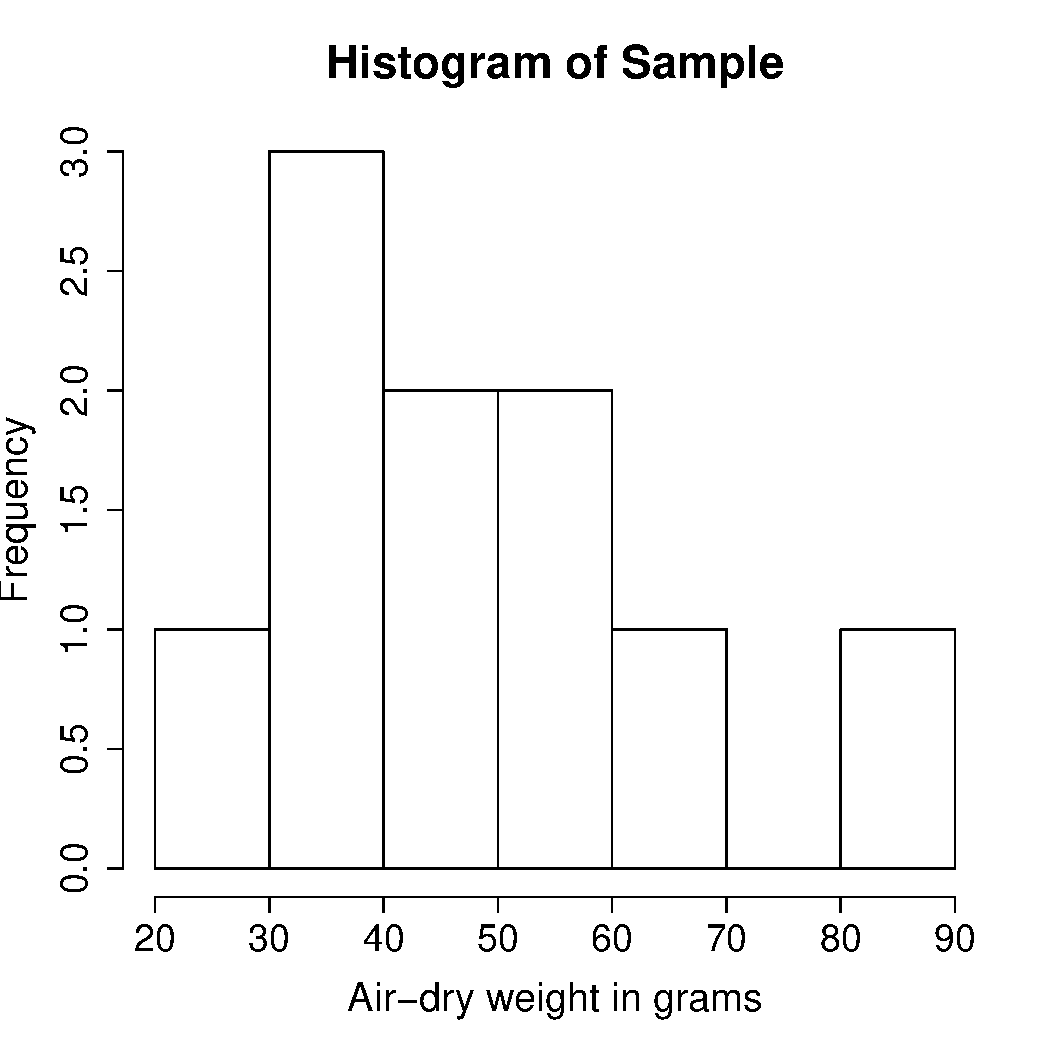
\includegraphics[width=\textwidth]{wgt_sample.pdf}
\end{minipage}
\begin{minipage}{.49\textwidth}
  We are assuming that the sample size $n=10$ and the difference $N-n = 716$ are large enough so that the Finite Central Limit theorem applies and that normal approximation practically approximates the distribution of $\hat \tau$.

  The histogram on the left shows that the sample distribution is not wildly skewed, so the convergence is likely sufficient for the scale of our sample.
\end{minipage}

\end{solution}

\subproblem{If you were charged with selecting a simple random sample of ten $3'\times2'$ plots from such a section, how would you do it?  Be specific.}

\begin{solution}
  As mentioned before, there are $N=726$ possible plots to sample. One could label them on a gridded map in a systematic way (say first by row, then column).  Then, using a random number generator that samples from $\{1,2,\dots,726\}$, one could obtain sample of indices, which in turn gives a sample of plots from the section.
\end{solution}

\subproblem{Estimate how big a sample of plots would be required to estimate the total biomass of the \unit[0.1]{acre} section to within a margin of error of \unit[3]{kg} with \unit[95]{\%} confidence.}

\begin{solution}
  If we think of the previous sample as a pilot study in which we are confident that $\sigma^2 \approx 325.38$, then the minimum sample size required to satisfy $P(|\hat \tau - \tau| > 3000) < .05$ is given by 
  $$
    n = \left(\frac 1N + \frac{d^2}{N^2\sigma^2z^2}\right)^{-1} = 66.50
  $$
  hence a sample of size of 67 would be sufficient. Based on our confidence of the estimate of $\sigma^2$, we may increase this.

\end{solution}

\problem{\textit{Thompson 4.1.} A botanical researcher wishes to design a survey to estimate the number of birch trees in a study area.  The study area has been divided into 1000 units or plots.  From previous experience, the variance in the number of stems per plot is known to be approximately $\sigma^2 \approx 45$. Using simple random sampling, what sample size should be used to estimate the total number of trees in the study area to within 500 trees of the true value with \unit[95]{\%} confidence?  To within 1000 trees? To within 2000 trees? }

\begin{solution}

\begin{minipage}{.3\textwidth}
\begin{tabular}{|c| c c|}
$d$ & $n$  & $n_0$\\\hline
500 & 409   &692\\
1000 & 148  &173\\
2000 & 42   &44 \\
\end{tabular}
\end{minipage} 
\begin{minipage}{.65\textwidth}
The table summarizes the calculations for both \textit{Thompson 4.1.~and 4.2.}
The calculation of $n$ was done similarly as in \textbf{3.}  Each $n_0$ is the second term in the denominator of calculating $n$.
\end{minipage}
\end{solution}

\problem{\textit{Thompson 4.2.} Compare the sample sizes for \textit{Thompson 4.1.} when the finite population correction factor is ignored.  What do you conclude about the importance of the finite population correction factor for this population? }

\begin{solution}
  If high precision is necessary in estimating the total, i.e.~d is on the order of 500, then the finite population correction factor gives a significantly lower bound than the naive bound.  Although, both cases may not be practical, since they are near a half of the total population and the convergence of the finite central limit theorem might break down.  For the less precise schemes, the correction makes less of a difference.
\end{solution}

\problem{\textit{Thompson 2.4.} Show that $E\left(s^2\right) = \sigma^2$ in simple random sampling, where the sample variance $s^2$ is defined with $n-1$ in the denominator and the population variance $\sigma^2$ is defined with $N-1$ in the denominator. Use the following two strategies. Write $y_i - \bar y$ as $y_i-\mu-(\bar y - \mu)$, verify that
$$
  \sum_{i=1}^n(y_i-\bar y)^2 = \sum_{i=1}^n(y_i - \mu)^2 - n(\bar y - \mu)^2
$$
and compute the expectation in two ways: 1) Take expectation over all possible samples and 2) defining an indicator variable for each unit, indicating whether it is included in the sample and computing the expectation of their sum.
}
\begin{solution}
  To verify the general identity given in the hint, we square then sum both sides of the equality, i.e.
  $$
    (y_i - \bar y)^2 = (y_i - \mu)^2 -2(y_i-\mu)(\bar y - \mu) + (\bar y - \mu)^2
  $$
  so
  \begin{align*}
    \sum_{i=1}^n (y_i - \bar y)^2 
    &= \sum_{i=1}^n (y_i - \mu)^2 -2(\bar y - \mu) \sum_{i=1}^n(y_i-\mu) + n(\bar y - \mu)^2 \\
    &= \sum_{i=1}^n (y_i - \mu)^2 -2(\bar y - \mu)(n\bar y-n\mu) + n(\bar y - \mu)^2 \\
    &=\sum_{i=1}^n (y_i - \mu)^2 - n(\bar y - \mu)^2.
  \end{align*}

  Now, let us adopt the notation that elements of the population are given by $y_1,y_2,\dots,y_N$, and for a given sample of indices $I$ of size $n$, the sample is $y_{I1},y_{I2},\dots,y_{In}$.  Further denote the realized sample mean and sample variance of $I$ as
  $$
    \bar y_I = \frac 1n	\sum_{i=1}^n y_{Ii}
    \quad\text{and}\quad
    s^2_I = \frac1{n-1}\sum_{i=1}^n (y_{Ii} - \bar y_I)^2.
  $$
  In an SRS, each sample is equally likely so $\displaystyle P(I) = \left. 1 \middle/ \binom N n\right.$. Then, using the same counting argument in calculating $\Var(\bar y)$ to rearrange the double summation, we have
  \begin{align*}
    E(s^2) &= \sum_{I \in \mathcal I} s^2_{I}P(I) \\
    &= \sum_{I \in \mathcal I} \left(\frac1{n-1}\sum_{i=1}^n (y_{Ii} - \bar y_I)^2\right)\left. \middle/ \binom Nn \right. \\
    %&= \frac1{n-1}\left(\sum_{i=1}^n (y_{Ii} - \bar y_I)^2\right)\left.\binom{N-1}{n-1} \middle/ \binom Nn \right. \\
    &= \left(\frac 1{n-1}\sum_{I \in \mathcal I} \sum_{i=1}^n (y_{Ii} - \mu)^2 - \frac n{n-1} \sum_{I\in \mathcal I}(\bar y_I - \mu)^2\right)\left. \middle/ \binom Nn \right. \\
    &= \left(\frac 1{n-1}\binom{N-1}{n-1}\sum_{i=1}^N (y_{Ii} - \mu)^2 - \frac n{n-1}\binom Nn \Var(\bar y)\right)\left. \middle/ \binom Nn \right. \\
    &= \frac 1{n-1}\frac nN(N-1)\sigma^2 - \frac {\cancel n}{n-1}\left(\frac{N-n}{N}\right)\frac{\sigma^2}{\cancel n} \\
    &= \sigma^2\left(\frac {nN-n - N -n}{(n-1)N}\right)\\
    &= \sigma^2.
  \end{align*}

  Now, let $Z_i\sim\mathrm{Bernouli}(\pi_i)$ indicate whether the population element $y_i$ is in a random sample where the inclusion probability is $ \pi_i = \left. \binom{N-1}{n-1} \middle/ \binom{N}{n}\right. = \frac nN$. Using the hint, then the linearity of expectation and that $\mu = E(\bar y_I)$ (i.e.~it is unbiased), we can write
  \begin{align*}
    (n-1)E\left(s^2_I\right) 
    &= E\left(\sum_{i=1}^n(y_{Ii} - \mu)^2 - n(\bar y_I - \mu)^2\right)\\
    &= \sum_{i=1}^NE\left(Z_i(y_i - \mu)^2\right) - n E\left((\bar y_I - \mu)^2\right)\\
    &= \sum_{i=1}^N\frac nN(y_i - \mu)^2 - n \Var(\bar y_I)\\
    &= \frac {n(N-1)\sigma^2}N - \cancel n \left(\frac{N - n}N\right)\frac{\sigma^2}{\cancel n}\\
    &= \sigma^2\left(\frac {nN-n - N -n}N\right)\\
    &= (n-1)\sigma^2,
  \end{align*}
  and canceling $n-1$ on both sides gives the desired equality.

\end{solution}

\begin{longproblem}
Suppose you would like to take an SRS of size $n$ from a list of $N$ units, but do not know the population size $N$ in advance.  Consider the following procedure:
\begin{enumerate}[(a)]
  \item Set $S_0 = \{1,2,\dots,n\}$, so that the initial sample for consideration consists of the first $n$ units on the list.
  \item For $k=1,2,\dots,$ generate a random number $u_k$ between $0$ and $1$.  If $u_k > n/(n+k)$, then set $S_k$ equal to $S_{k-1}$.  If $u_k\le n/(n+k)$, then select one of the units in $S_{k-1}$ at random, and replace it by unit $(n+k)$ to form $S_k$.
\end{enumerate}
Show that $S_{N-n}$ from this procedure is an SRS of size $n$. \emph{Hint:} Use induction.
\end{longproblem}
\begin{solution}
   Fix the sample size at $n$, and let $k=N-n$ be the difference in the size
   between the population to the sample.
   For clarity, denote $S_k:\Omega \to \{1,2,\dots,(n+k)\}^n$ a random variable whose realizations are denoted $S_k(\omega) = s_k$.  
   %Denote $S_k$ to be the random sample of indices from $1,2,\dots,(n+k)$
   %obtained on the $k$th step of the algorithm and $s_k$ its realization.  
   We must show that $S_k$ takes on each subset of $\{1,2,\dots,N=n+k\}$ of size $n$ with equal probability.  We proceed by induction on $k$ from
   $k=0$ to $k=N-n$.

   In the base case, $k=0$ implies $N=n$ and $S_0$ takes on only $s_0 =
   \{1,\dots,n\}$ with probability 1, which is the only subset of $\{1,\dots,N=n+0\}$ of size $n$. Hence it is trivally a
   random sample of all such subsets.

  Now, assume the induction hypothesis, i.e.~$S_k$ produces an SRS for a population of size $n+k$ -- equivalently,
  $$
   P(S_k = s_k) = \left. 1 \middle/ \binom{n+k}{n} \right.
  $$
  for each subset $s_k$ of size $n$ from $\{1,2,\dots,(n+k)\}$.
  Upon the realization $S_{k+1}=s_{k+1}$, either the sample remains fixed with $S_{k+1} = s_k$, in which case
   $u_{k+1} \in \left(\frac
  n{n+k+1},1\right)$ with probability $\left( 1 - \frac{n}{n+k+1}\right)=\left(
  \frac{k+1}{n+k+1} \right)$, or $S_{k+1}$ takes on $s_k$ with a randomly selected element replaced with
  $(n+k+1)$, in which case $u_{k+1} \in \left(0,\frac n{n+k+1}\right]$
  with probability $\left( \frac{k+1}{n+k+1} \right)$. If we assume that the
  selection of $u_{k+1}$ is independent of the generation of the sample from
  the previous step, then in the first case
  \begin{align*}
    P(S_{k+1} = s_{k+1}) 
    &= P(S_k = s_k) P\left(U_{k+1} \in \left(\frac n{n+k+1},1\right) \right) \\
    &=\binom {n+k}{n}^{-1} \left( \frac{k+1}{n+k+1} \right)\\
    &=\binom {n+k+1}n^{-1}
  \end{align*}
  In the second case, denote $s_k =\{a_1,a_2,\dots,a_n\}$, then $s_{k+1} =
  s_k\setminus\{a_i\}\cup\{k+1+n\}$ where $a_i$ is the realization of the
  random selection in the algorithm.  For each event where
  $\{a_1,a_2,\dots,a_n\}\setminus a_i \subset S_k$, there are $(n+k) - (n-1) = k+1$
  possible choices that fix each $a_1,\dots,a_n$ except for $a_i$.  Since each
  of those events are disjoint and have equal probability, $P(S_{k+1} = s_{k+1}
  | u_k,a_i) = P(\{a_1,\dots,a_n\}\setminus a_i \in S_k) = (k+1)\binom{n+k}n^{-1}$.  Now, assuming the independence
  of realization of $u_k$ and $a_i$ and the previous selection, we have
  \begin{align*}
    P(S_{k+1} = s_{k+1}) &= \left((k+1)\binom{n+k}n^{-1}\right)\cdot P\left(U_{k+1} \in \left(0,\frac n{n+k+1}\right] \right) \cdot P\Big( A_i = a_i \Big)\\
    &= (k+1)\binom{n+k}n^{-1}\cdot \frac n{n+k+1} \cdot \left( \frac 1n\right)\\
    &= \binom{n+k}{n}^{-1}\frac{k+1}{n+k+1}\\
    &=\binom {n+k+1}n^{-1}.
  \end{align*} 
\end{solution}
\end{document} 


